\chapter{Antenne su piano conduttore}

Nei capitoli precedenti abbiamo osservato che piani composti da \gls{pec} si comportano come specchi per l'onda elettromagnetica, avendo coefficiente di riflessione $\rho = 1$.
Osserviamo quindi come questi specchi di \gls{pec} possano essere sfruttati come elementi attivi per le antenne.

\section{Teorema delle immagini}

In presenza di un piano infinito di \gls{pec}, come in \autoref{fig:piano_di_massa}, il teorema delle immagini afferma che il campo prodotto da una sorgente di campo elettromagnetico $I \Delta z_{(1)}$ risulta uguale al campo prodotto da un sistema privato dello specchio e composto dalla sorgente stessa e dalla sua versione ``riflessa'' $I \Delta z_{(2)}$.

\begin{figure}[htp]
	\centering
	\begin{subfigure}{.45\textwidth}
		\centering
		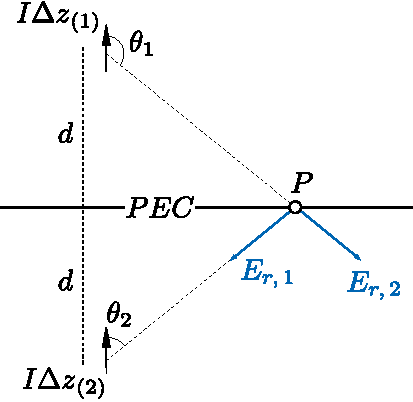
\includegraphics[]{img/piano_di_massa_r.pdf}
		\caption{}
		\label{fig:piano_di_massa_r}
	\end{subfigure}\hfill%
	\begin{subfigure}{.45\textwidth}
		\centering
		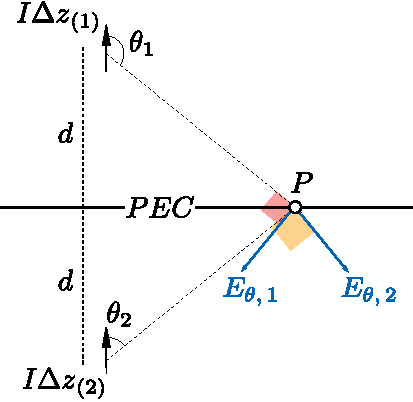
\includegraphics[]{img/piano_di_massa_theta.pdf}
		\caption{}
		\label{fig:piano_di_massa_r}
	\end{subfigure}
	\caption{Il campo lungo le due componenti risulta perpendicolare al piano, come richiesto dalle condizioni al contorno.}
	\label{fig:piano_di_massa}
\end{figure}

Per poter affermare questa equivalenza bisogna soddisfare le condizioni al contorno: in questo caso quindi il campo tangente al piano di \gls{pec} deve annullarsi, sia la componente lungo $\hat{r}$ che quella lungo $\hat{\theta}$.

Dato un opportuno coefficiente $C$ di proporzionalità, possiamo scrivere il campo radiale come
\begin{equation}\begin{dcases}
	\E_{r,\, 1} = C \cos(\theta_1)\hr_1 \\
	\E_{r,\, 2}
	= C \cos(\theta_2)\hr_2
	= C \cos(\pi - \theta_1) \hr_2
	= -C \cos(\theta_1) \hr_2 \\
\end{dcases}\end{equation}
dove $C$ è uguale nelle due espressioni per la simmetria del sistema.

La componente del campo lungo $\hat{\theta}$ vale invece
\begin{equation}\begin{cases}
	\E_{\theta_1}
	= D \, \sin(\theta_1) \hth_1 \\
	\E_{\theta_2}
	= D \, \sin(\theta_2)\hth_2
	= D \, \sin(\theta_1) \hth_2 \\
\end{cases}\end{equation}
dove il coefficiente di proporzionalità $D$ è uguale, sempre per simmetria.

Il campo risultante per entrambe le componenti risulta perciò perpendicolare al piano: data questa scelta di direzione, verso e intensità della sorgente riflessa lo schema risulta perciò equivalente a quello iniziale.

\clearpage
\section{Monopòli}

Per il teorema delle immagini, lo specchio introduce un effetto che può essere interpretato come un'antenna virtuale: sfruttiamo ora questo principio per costruire dei \emph{monopoli elettromagnetici}.

Si tratta di comuni dipoli elettrici, in cui però uno dei due morsetti è collegato al piano conduttore.

L'impedenza, la resistenza di radiazione e la potenza di trasmissione del monopolo sono quindi analoghi al caso studiato in precedenza, ma, data la mancanza di metà dell'antenna, l'impedenza d'antenna e la potenza irradiata dimezzano.

\begin{esp}
	Z_{monopolo}
	&= \frac {V_A}{2} \, \frac{1}{I_A}
	= \frac{1}{2} Z_{dipolo}\\
	R_{r, \,monopolo}
	&=\frac{1}{2} R_{r, \, dipolo}\\
	P_{monopolo}
	&= R_{r, \,monopolo} \, \frac{|I_A|^2}{2}
	= \frac{P_{dipolo}}{2}
\end{esp}

Nel caso del monopolo corto, in particolare si ha che che la resistenza dimezza, come anticipato sopra con l'impedenza, ma la direttività raddioppia, essendo il campo concentrato solamente \emph{al di sopra} del piano conduttore.

\begin{esp}
	R_{r, \, monopolo}
	&= \frac{\pi}{12}\eta\left(\frac{L}{\lambda}\right)^2
	\simeq 40 \pi^2 \left(\frac{L}{\lambda}\right)^2 \\
	D_{monopolo}
	&= \frac{4\pi U_m}{P_{monopolo}}
	= \frac{4\pi U_m}{\frac{P_{dipolo}}{2}}
	= 2 D_{dipolo}
\end{esp}

\section{ILA - Inverted L antenna}
Questo tipo di antenna corta prende il nome dalla sua forma a L rovesciata.

L'idea alla base di questa particolare forma è che, osservando la \autoref{fig:ila}, la sezione orizzontale concentra su di sè i valori di corrente più bassa, perché vicina al punto stazionario all'estremità.

\begin{figure}[htp]
	\centering
	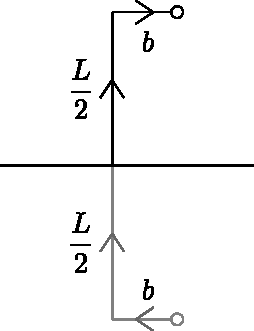
\includegraphics[]{img/ila.pdf}
	\caption{Antenna ILA con la sua sua controparte virtuale. Il punto stazionario è marcato con un cerchio, mentre il verso delle correnti con frecce lungo i segmenti.}
	\label{fig:ila}
\end{figure}

Nella sezione verticale, che effettivamente irradia nel campo lontano, la densità di corrente elettrica sarà perciò maggiore, incrementando le prestazioni.

\smallbreak
Cerchiamo quindi di di calcolare il momento del dipolo magnetico per questa antenna.

\begin{esp}
	\M(\theta,\Phi)
	&\stackrel{(1)}{\simeq} \int_{-\frac{L}{2}}^{\frac{L}{2}} I(z^{\prime}) \de z^{\prime} \\
	&\stackrel{(2)}{=} I_m
	\int_{-\frac{L}{2}}^{\frac{L}{2}}
	\left(
		1-\frac{|z^{\prime}|}{\frac{L}{2}+b}
	\right)
\de z^{\prime} \\
	&= I_m\left(L- \int_0^{\frac{L}{2}}\frac{z^{\prime}}{\frac{L}{2}+b} \de z^{\prime} + \int_{-\frac{L}{2}}^0\frac{z^{\prime}}{\frac{L}{2}+b} \de z^{\prime}\right)\\
	&=I_m \left(\left. L - \frac{(z^\prime)^2}{2 \cdot \left(\frac{L}{2}+b\right)} \right|_0^{\frac{L}{2}}+\left. \frac{(z^\prime)^2}{2 \cdot \left(\frac{L}{2}+b\right)} \right|_{-\frac{L}{2}}^0 \right)\\
	&=I_m \, \frac{4L\left(\frac{L}{2}+b\right)-L^2}{4\left(\frac{L}{2}+b\right)}
	= I_m \, \frac{L}{2} \,  \underbrace{\frac{L+4b}{L+2b}}_{>1}
\end{esp}
Quindi abbiamo ottenuto che
\begin{equation}
	M_{monopolo}
	= I_m \, \frac{L}{2} \,  \underbrace{\frac{L+4b}{L+2b}}_{>1}
	> I_m \, \frac{L}{2}
	= M_{dipolo}
\end{equation}

Le antenna a dipolo possono essere modificate anche in altri modi, per esempio nel caso in cui si voglia avere un'antenna più capacitiva si può mettere, al posto del ramo parallelo al PEC, un disco fatto con un buon conduttore.

\section{IFA - Inverted F antenna}

Le antenne IFA sono spesso usate nei cellulari in quanto la loro struttura è semplice, come si può vedere in \autoref{fig:ifa}.
Vengono utilizzate spesso negli smartphone in quanto permettono di sfruttare tutti gli spazi lasciati vuoti dalle altre componenti e sono antenne non molto direttive.
\begin{figure}[htp]
	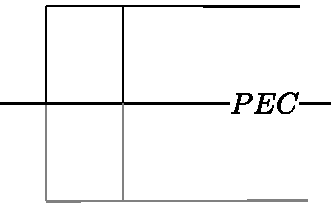
\includegraphics{img/ifa.pdf}
	\caption{Antenna IFA. La versione specchiata sul piano è resa in grigio.}
	\label{fig:ifa}
\end{figure}

%%% Local Variables:
%%% mode: latex
%%% TeX-master: "antenne"
%%% End:
